\documentclass[12pt,a4paper]{article}
% =============================================================================
% PAPER B — Cortes em educação e desigualdade regional no Brasil
% Painel das 27 UF + projeção regional de um choque fiscal educacional
% =============================================================================
\usepackage[utf8]{inputenc}
\usepackage[T1]{fontenc}
\usepackage[brazil]{babel}
\usepackage{mathptmx}
\usepackage{geometry}
\geometry{a4paper,left=1.8cm,right=1.8cm,top=2cm,bottom=2cm}
\usepackage{setspace}
\singlespacing
\usepackage{graphicx}
\usepackage{float}
\usepackage{booktabs}
\usepackage{array}
\usepackage{tabularx}
\usepackage{caption}
\usepackage{subcaption}
\usepackage{amsmath,amssymb}
\usepackage{enumitem}
\usepackage[round,authoryear]{natbib}
\bibliographystyle{plainnat}
\usepackage{xcolor}
\usepackage[colorlinks=true,linkcolor=black,citecolor=blue!50!black,urlcolor=blue!50!black]{hyperref}
\renewcommand{\tablename}{Tabela}
\renewcommand{\figurename}{Figura}
\renewcommand{\bibname}{Refer\^encias}
\captionsetup{font=small,labelfont=bf,justification=centering}
\newcolumntype{Y}{>{\arraybackslash}X}
\newcommand{\fonte}[1]{\captionsetup{font=scriptsize}\caption*{\footnotesize Fonte: #1}}

\title{\textbf{Cortes em Educa\c{c}\~ao e Desigualdade Regional no Brasil:}\\[2pt]
\textbf{\large Evid\^encias em Painel das 27 UF e a Incid\^encia Espacial de um Choque Fiscal Educacional}}
\author{Valber Gregory Barbosa Costa Bezerra Santos\thanks{Universidade Federal de Alagoas (UFAL) -- Unidade Educacional de Penedo; Tribunal de Justi\c{c}a do Estado de Alagoas. E-mail: \texttt{valber.santos@penedo.ufal.br}. Para avalia\c{c}\~ao \`as cegas, suprimir esta nota.}}
\date{\today}

\begin{document}
\maketitle
\begin{center}\small
\textbf{\'Area ANPEC:} 10 -- Economia Regional e Urbana (aderente \`a 12 -- Economia Social).\\
\textbf{JEL:} I24; I28; J31; R11; R23; H75.
\end{center}

\begin{abstract}
% AUTHOR WRITES
\end{abstract}
% AUTHOR WRITES: Abstract

% =============================================================================
\section{Introdu\c{c}\~ao}
% AUTHOR WRITES
% =============================================================================

% =============================================================================
\section{Revis\~ao de literatura}
% AUTHOR WRITES
% =============================================================================

% =============================================================================
\section{Estrat\'egia emp\'irica e dados}\label{sec:emp}
% AUTHOR WRITES
% =============================================================================

\begin{table}[H]
\centering
\caption{Estat\'isticas descritivas (base calibrada, 27 UF $\times$ 13 anos)}
\label{tab:desc}
\small
\begin{tabular}{lrrrr}
\toprule
Variável & Média & Desvio & Mínimo & Máximo \\
\midrule
Salário médio (R\$) & 2.447,1 & 687,8 & 1.323,1 & 4.284,0 \\
Gasto educ. pc (R\$) & 735,8 & 185,9 & 383,1 & 1.736,9 \\
PIB pc (R\$) & 31.099,9 & 6.873,1 & 18.617,0 & 53.144,8 \\
\bottomrule
\end{tabular}

\fonte{Elabora\c{c}\~ao pr\'opria.}
\end{table}

\begin{figure}[H]
\centering
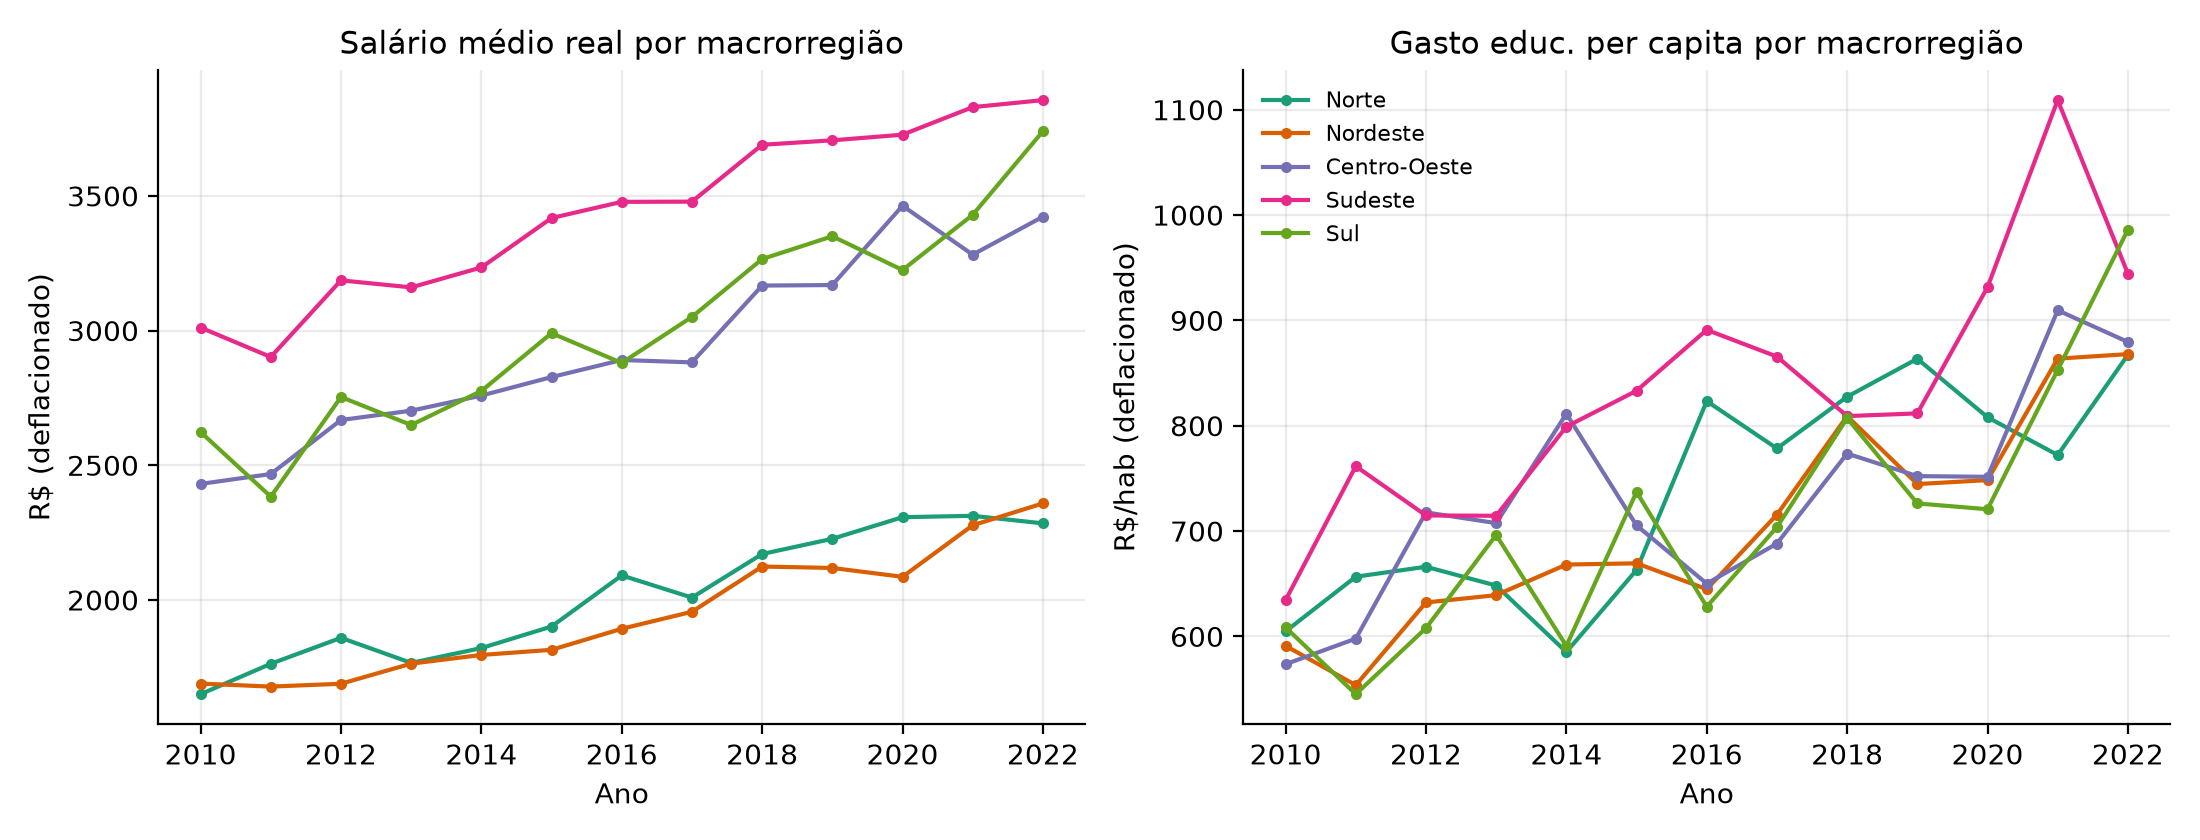
\includegraphics[width=\textwidth]{figures/evolucao_painel.png}
\caption{Evolu\c{c}\~ao do sal\'ario m\'edio real e do gasto educacional per capita por macrorregi\~ao}
\label{fig:evol}
\fonte{Elabora\c{c}\~ao pr\'opria.}
\end{figure}

% =============================================================================
\section{Resultados I: elasticidade e heterogeneidade regional}\label{sec:res1}
% AUTHOR WRITES
% =============================================================================

\begin{table}[H]
\centering
\caption{Modelo de efeitos fixos -- dependente: $\log$(sal\'ario m\'edio)}
\label{tab:fe}
\small
\begin{tabular}{lcccc}
\toprule
 & (1) Pooled & (2) FE 2-vias & (3) FE 2-vias & (4) FE entidade \\
 & OLS & Clustered & Driscoll-Kraay & + tendência \\
\midrule
$\log$(Gasto educ. pc) & 0.256*** & 0.173*** & 0.173*** & 0.175*** \\
 & (0.075) & (0.027) & (0.015) & (0.026) \\
$\log$(PIB pc) & 1.021*** & 0.387*** & 0.387*** & 0.411*** \\
 & (0.078) & (0.056) & (0.039) & (0.051) \\
\midrule
Efeitos fixos UF & Não & Sim & Sim & Sim \\
Efeitos fixos ano & Não & Sim & Sim & Não \\
Observações & 351 & 351 & 351 & 351 \\
$R^2$ (within) & -- & 0.603 & 0.603 & 0.833 \\
\bottomrule
\end{tabular}

\begin{minipage}{0.95\textwidth}\vspace{2pt}\scriptsize
Nota: erros entre par\^enteses. \textsuperscript{*}$p<0{,}10$; \textsuperscript{**}$p<0{,}05$; \textsuperscript{***}$p<0{,}01$. (1) \emph{pooled}; (2) FE clusterizado; (3) FE Driscoll--Kraay; (4) FE com tend\^encia.
\end{minipage}
\fonte{Elabora\c{c}\~ao pr\'opria.}
\end{table}

\begin{table}[H]
\centering
\caption{Elasticidade sal\'ario-educa\c{c}\~ao por macrorregi\~ao}
\label{tab:reg}
\small
\begin{tabular}{lcccc}
\toprule
Macrorregião & Elasticidade & Erro-padrão & $p$-valor & $N$ \\
\midrule
Norte & 0.206*** & 0.038 & 0.000 & 91 \\
Nordeste & 0.208*** & 0.056 & 0.000 & 117 \\
Centro-Oeste & 0.188*** & 0.039 & 0.000 & 52 \\
Sudeste & -0.009 & 0.086 & 0.919 & 52 \\
Sul & 0.155*** & 0.009 & 0.000 & 39 \\
\bottomrule
\end{tabular}

\fonte{Elabora\c{c}\~ao pr\'opria.}
\end{table}

\begin{figure}[H]
\centering
\begin{minipage}{0.49\textwidth}\centering
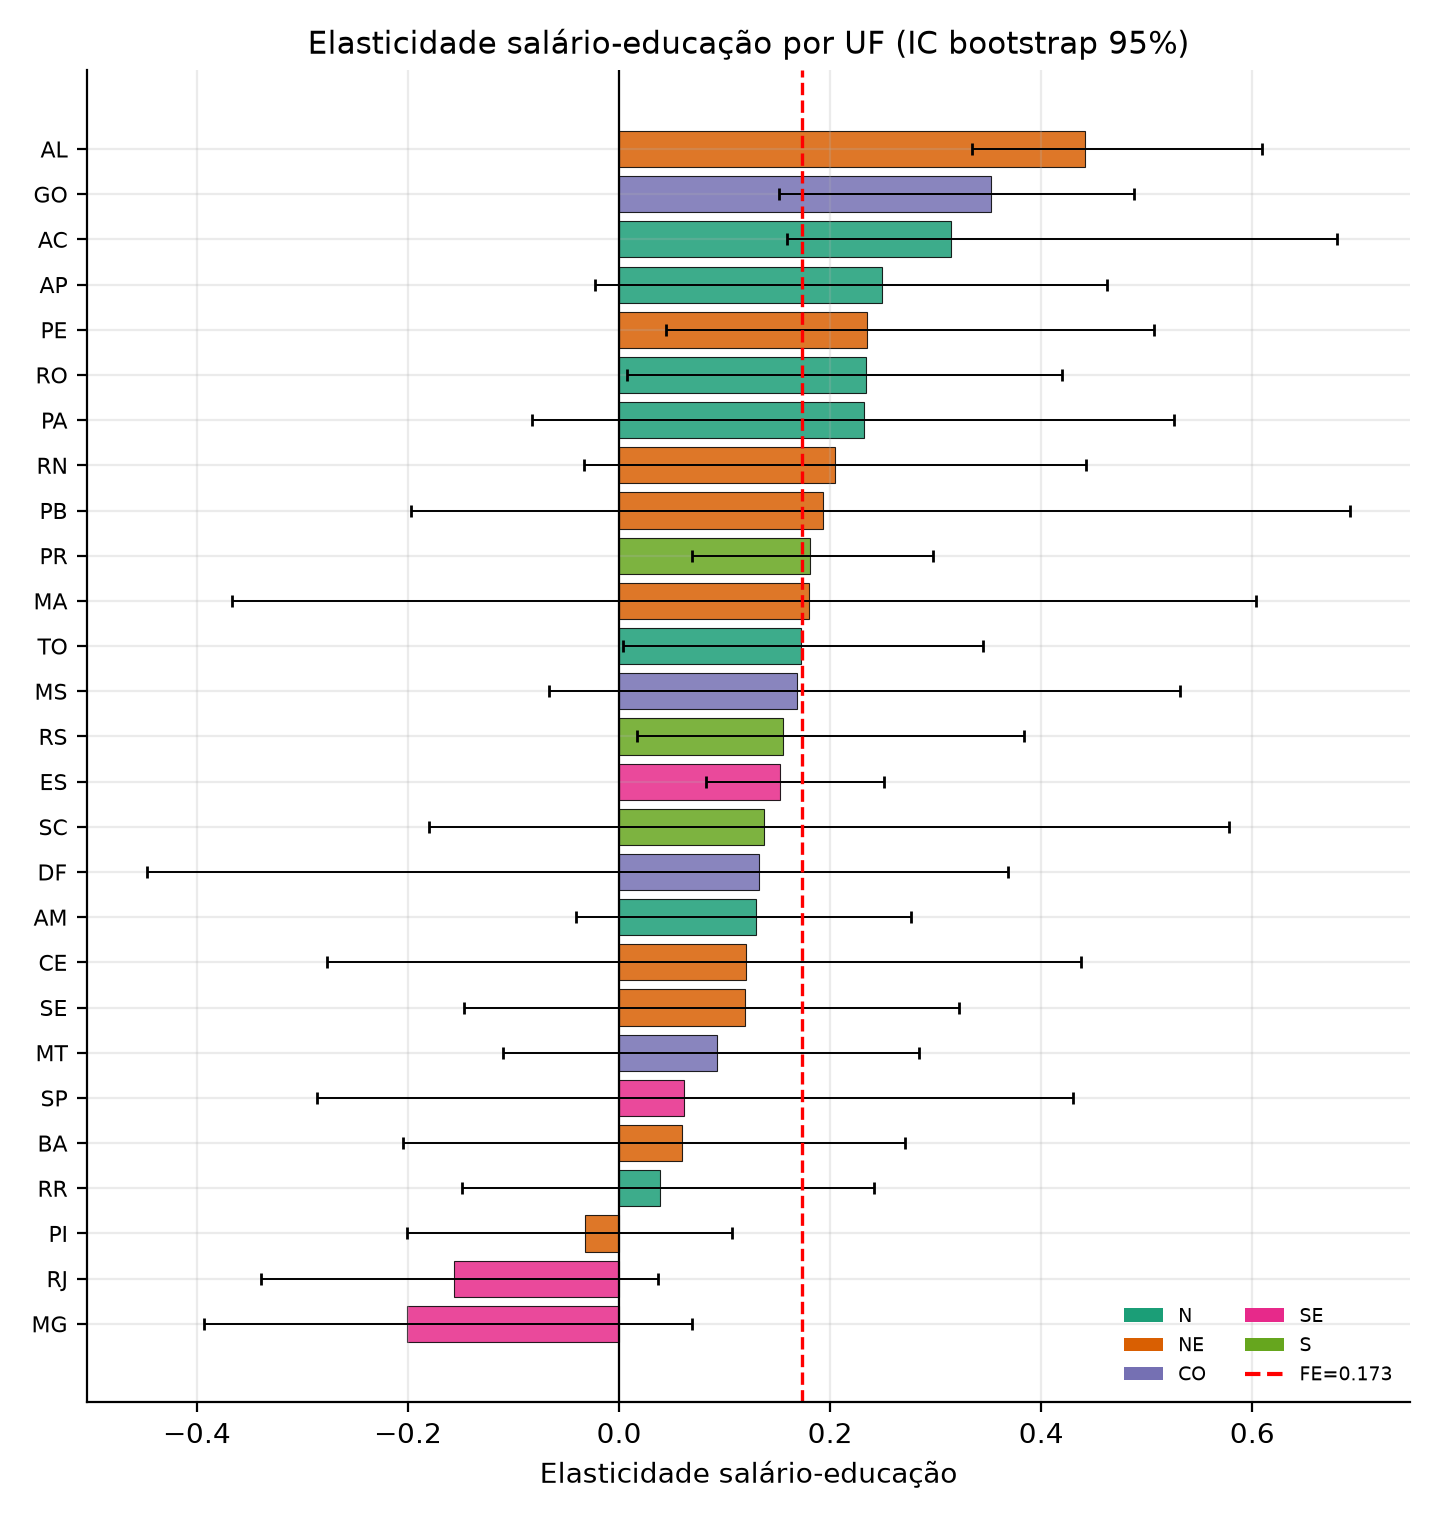
\includegraphics[width=\textwidth]{figures/elasticidade_uf_ic.png}
\end{minipage}\hfill
\begin{minipage}{0.49\textwidth}\centering
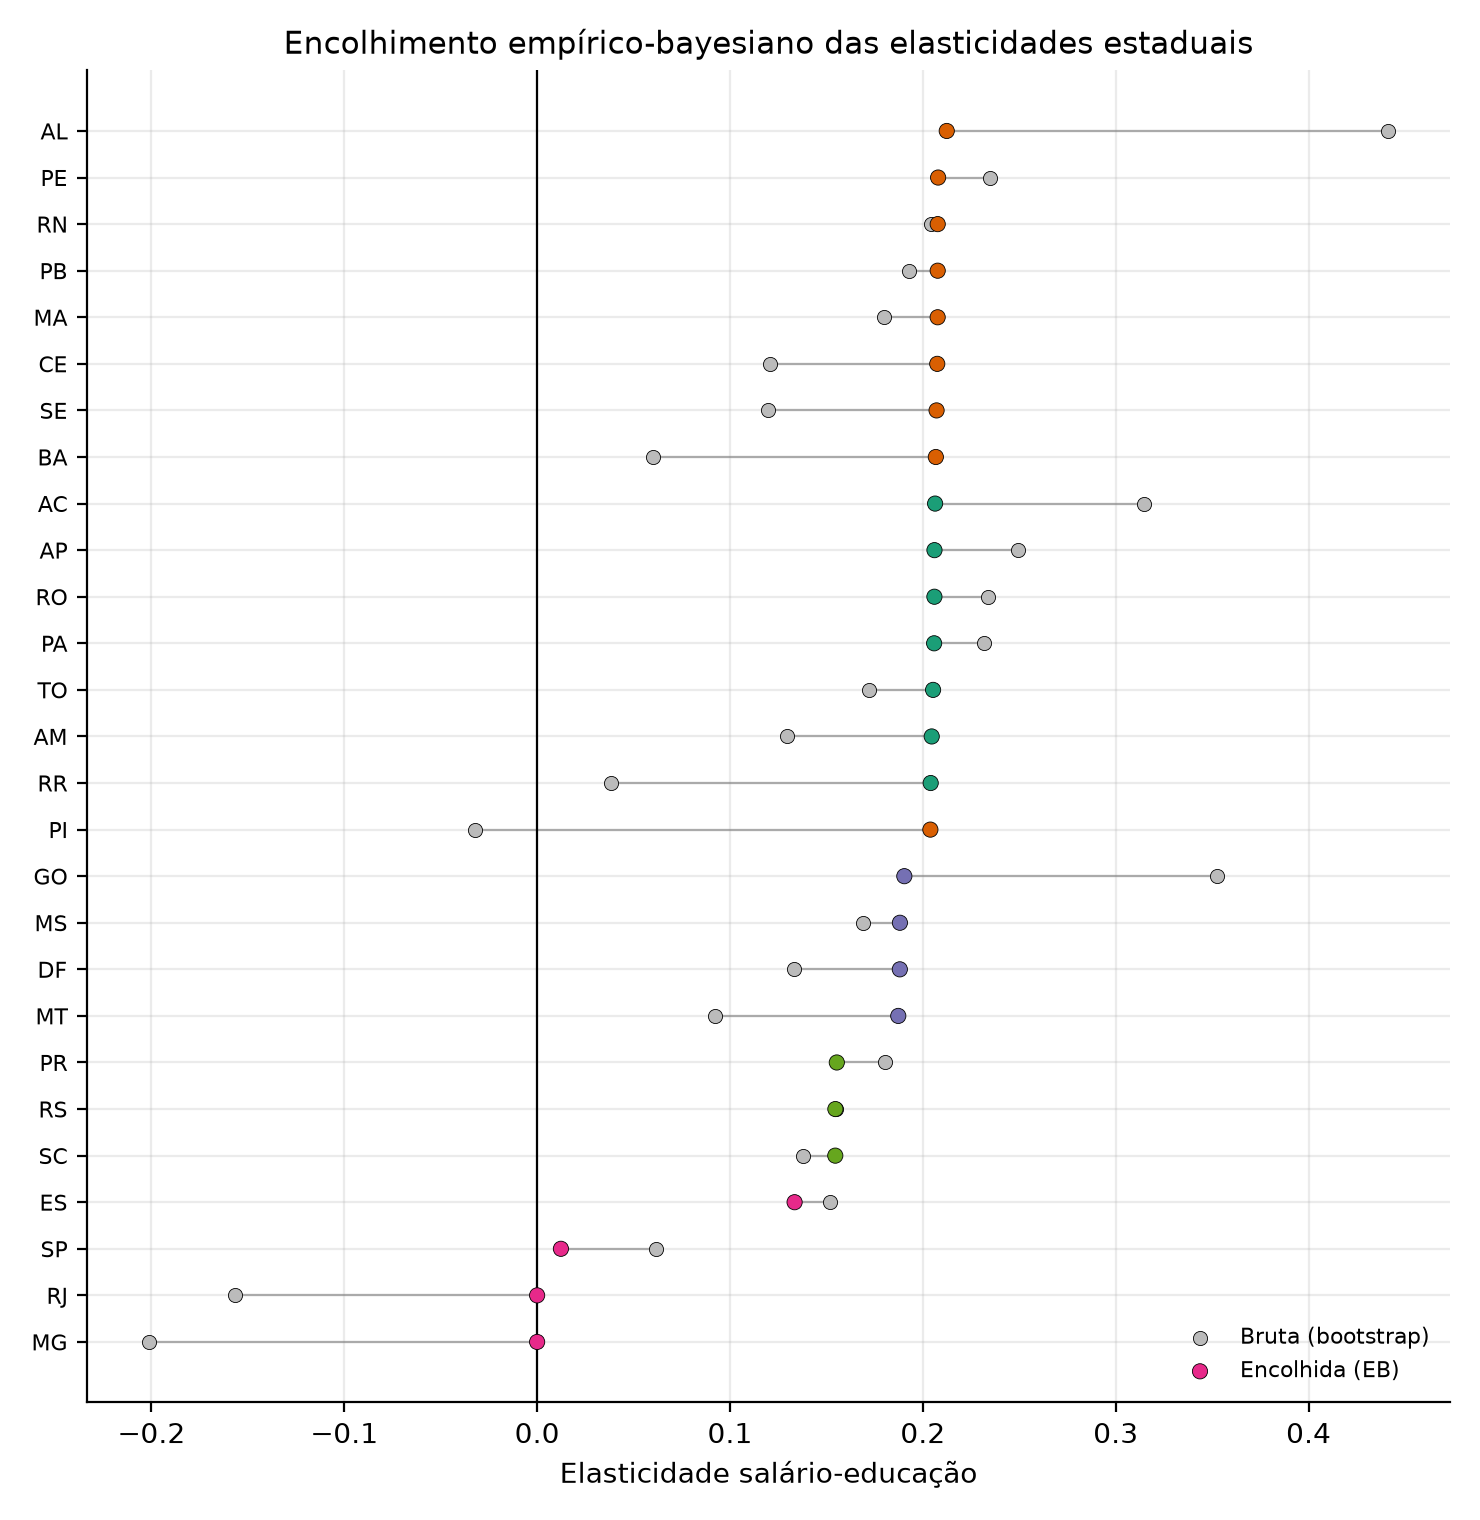
\includegraphics[width=\textwidth]{figures/encolhimento_eb.png}
\end{minipage}
\caption{Elasticidades estaduais com IC \emph{bootstrap} de $95\%$ (esq.) e encolhimento emp\'irico-bayesiano (dir.)}
\label{fig:eb}
\fonte{Elabora\c{c}\~ao pr\'opria.}
\end{figure}

\begin{figure}[H]
\centering
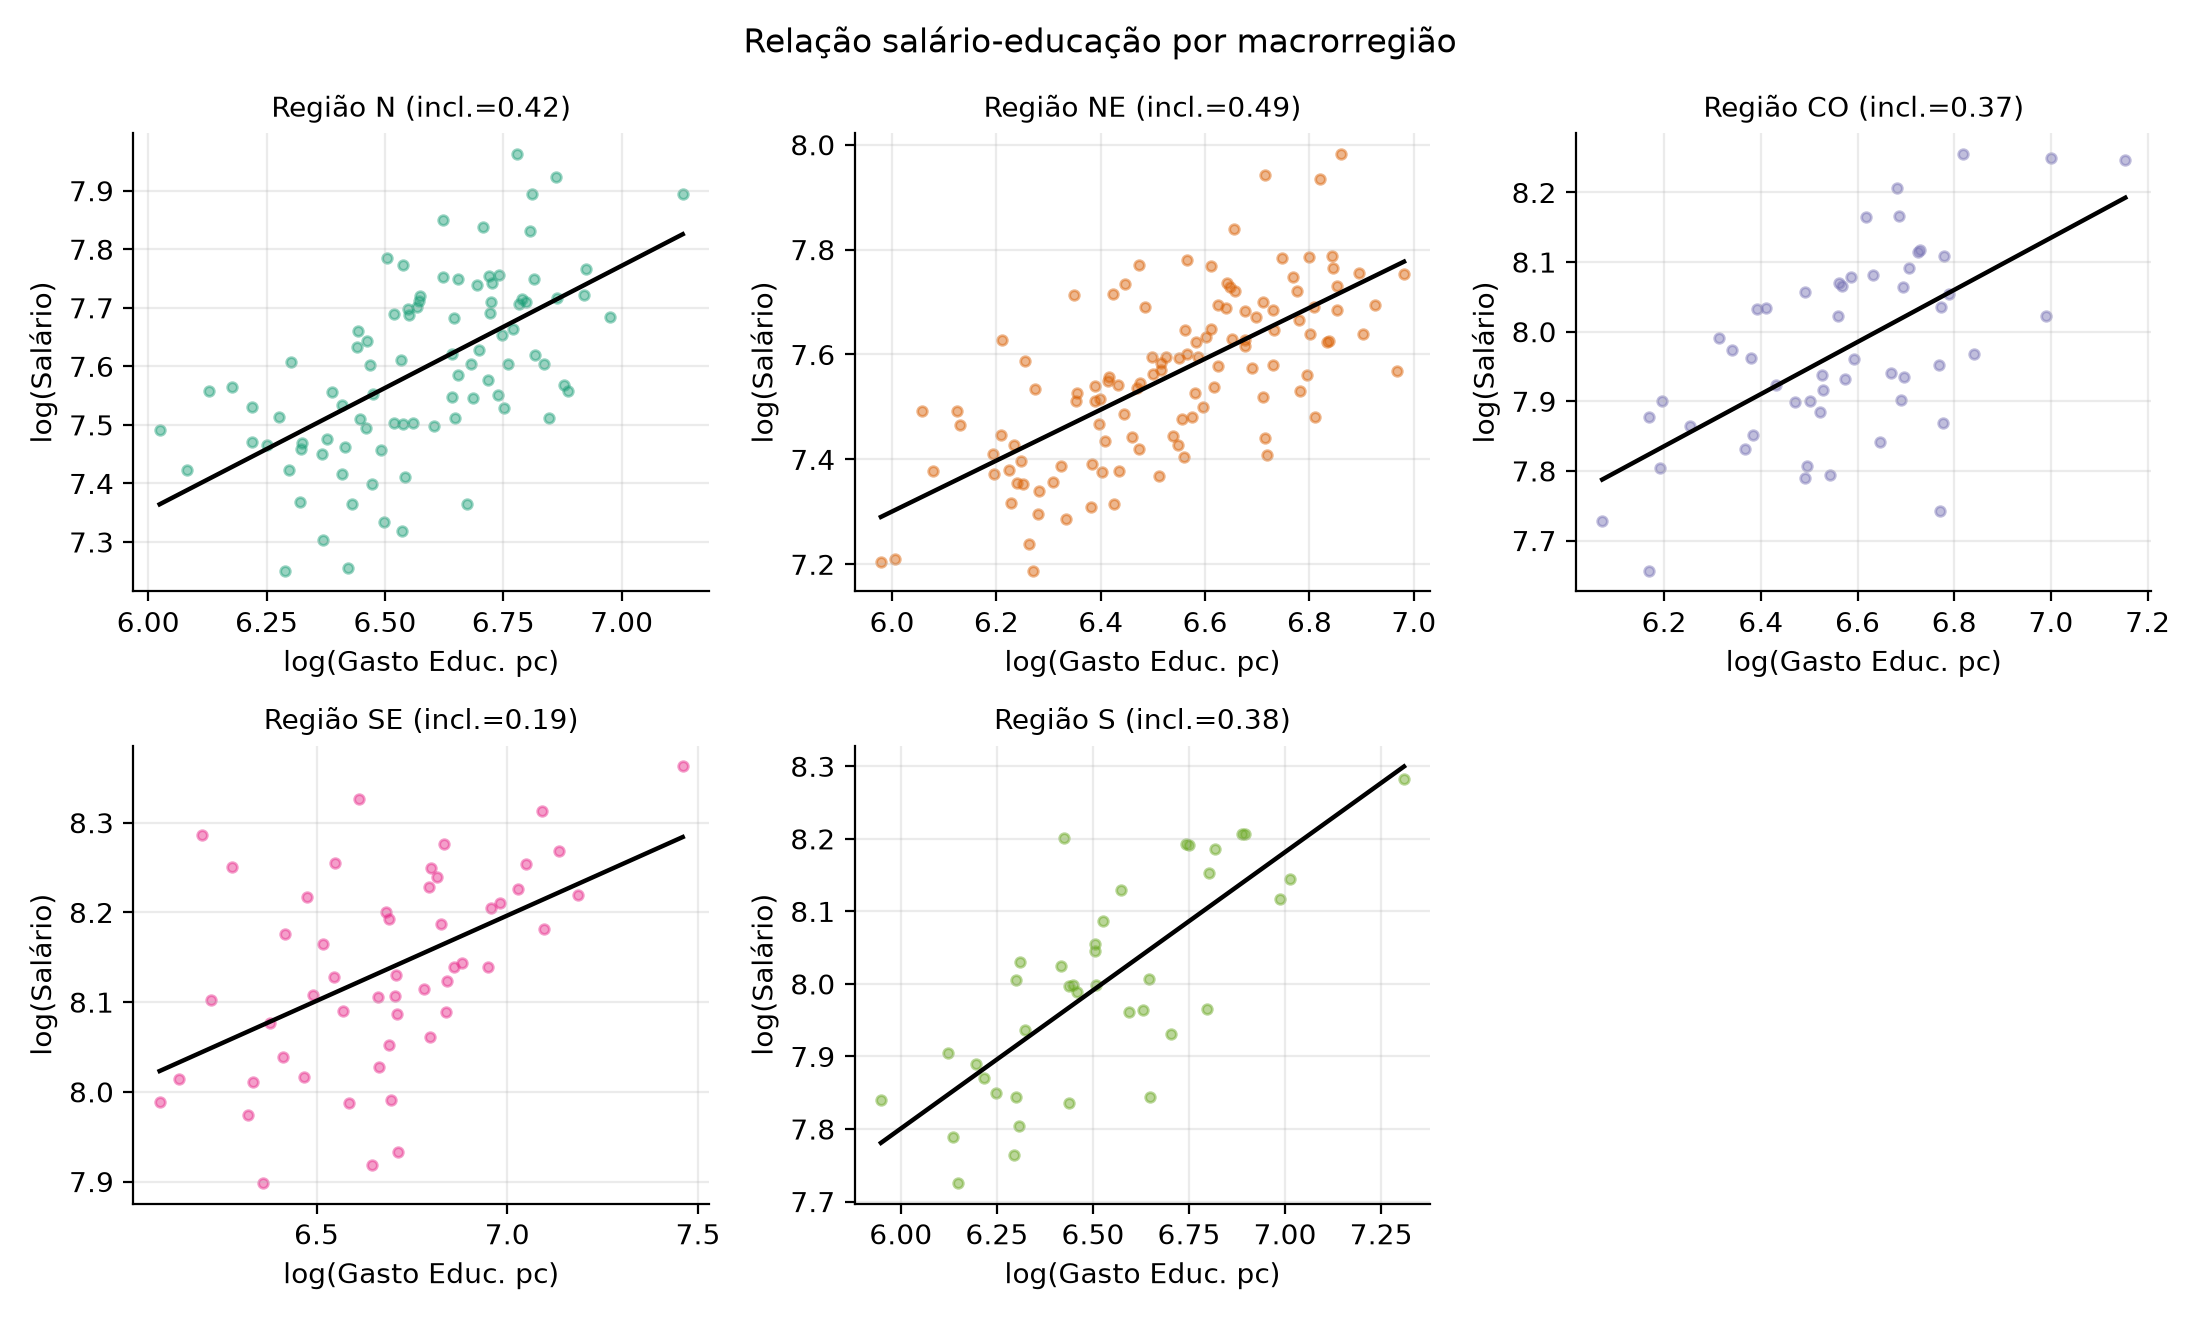
\includegraphics[width=0.9\textwidth]{figures/dispersao_uf.png}
\caption{Rela\c{c}\~ao sal\'ario-educa\c{c}\~ao por macrorregi\~ao}
\label{fig:disp}
\fonte{Elabora\c{c}\~ao pr\'opria.}
\end{figure}

% =============================================================================
\section{Resultados II: incid\^encia regional do corte}\label{sec:res2}
% AUTHOR WRITES
% =============================================================================

\begin{figure}[H]
\centering
\begin{minipage}{0.56\textwidth}\centering
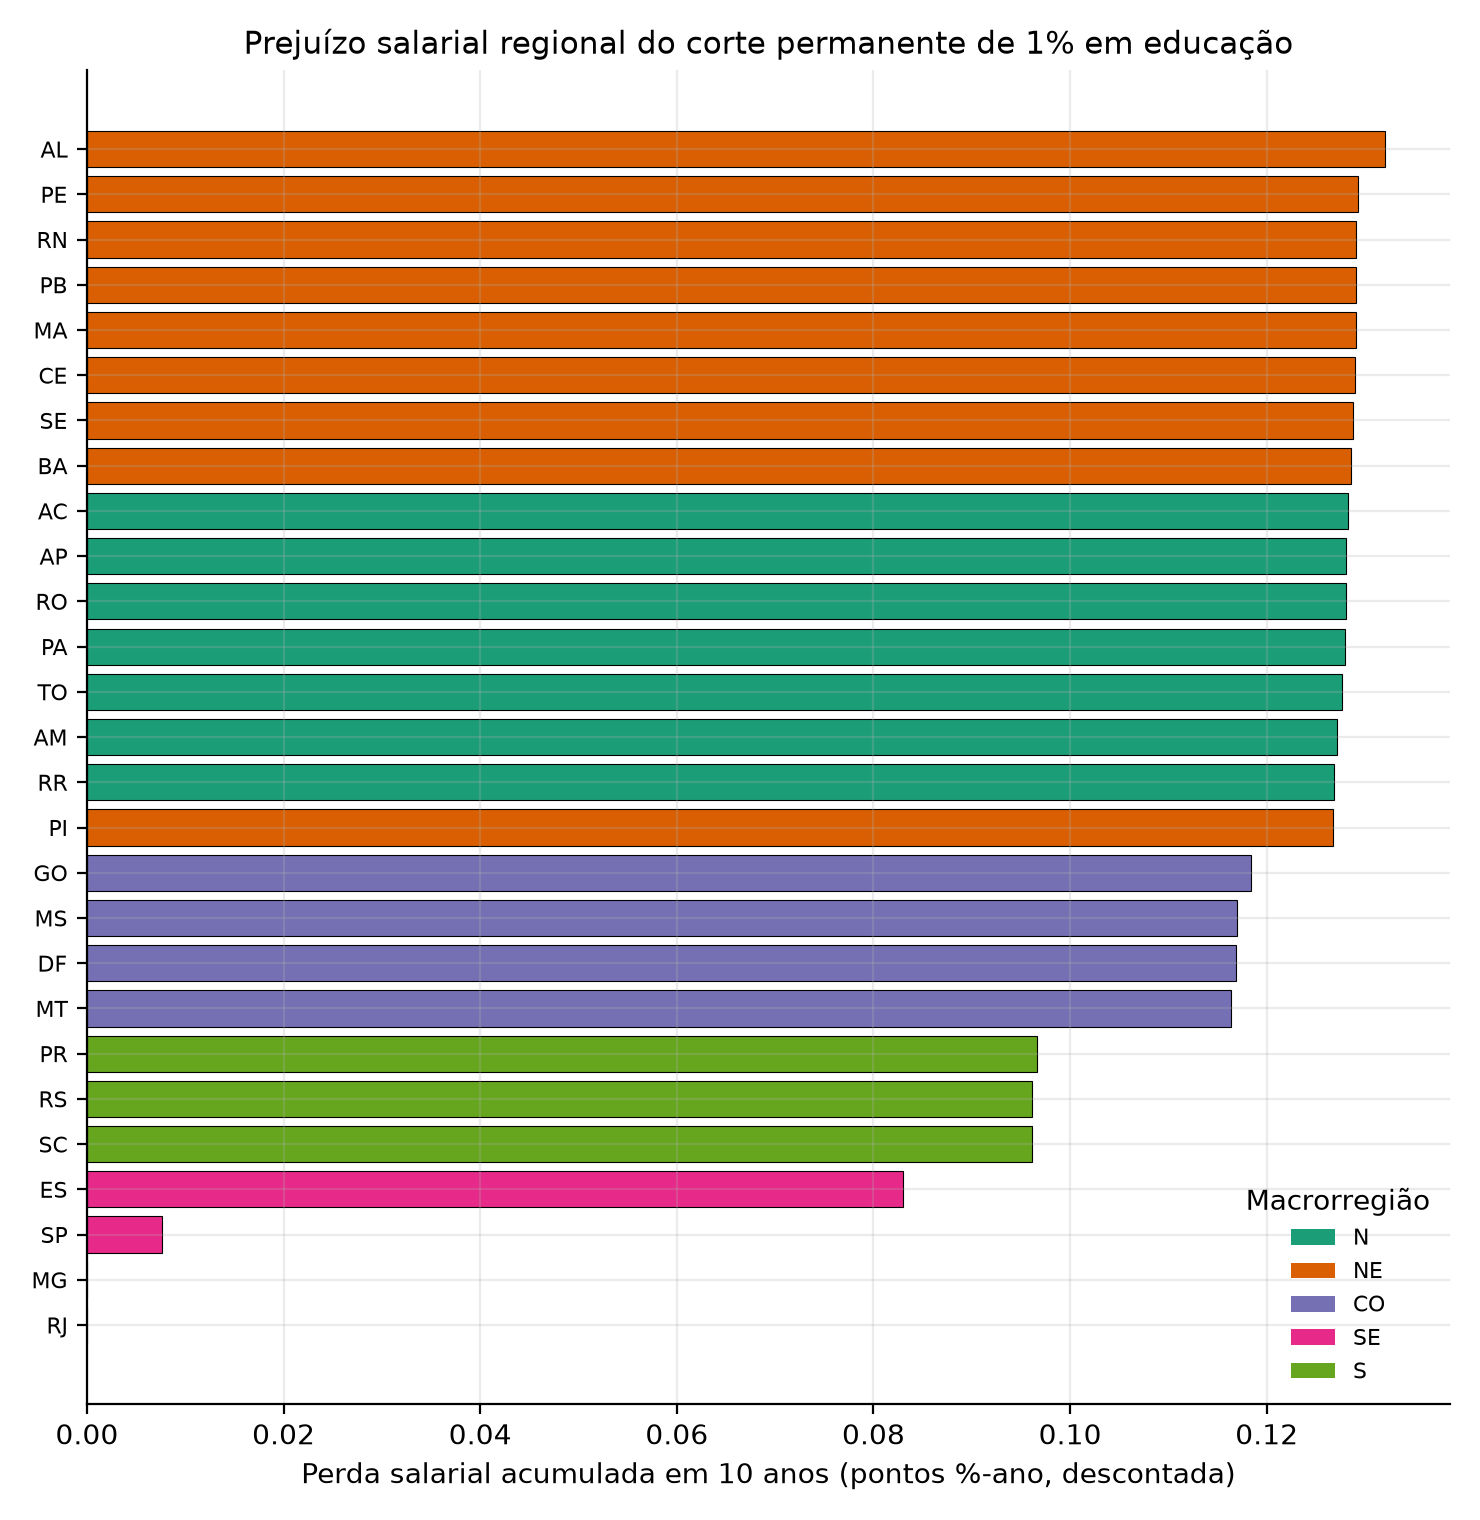
\includegraphics[width=\textwidth]{figures/projecao_regional.png}
\end{minipage}\hfill
\begin{minipage}{0.42\textwidth}\centering
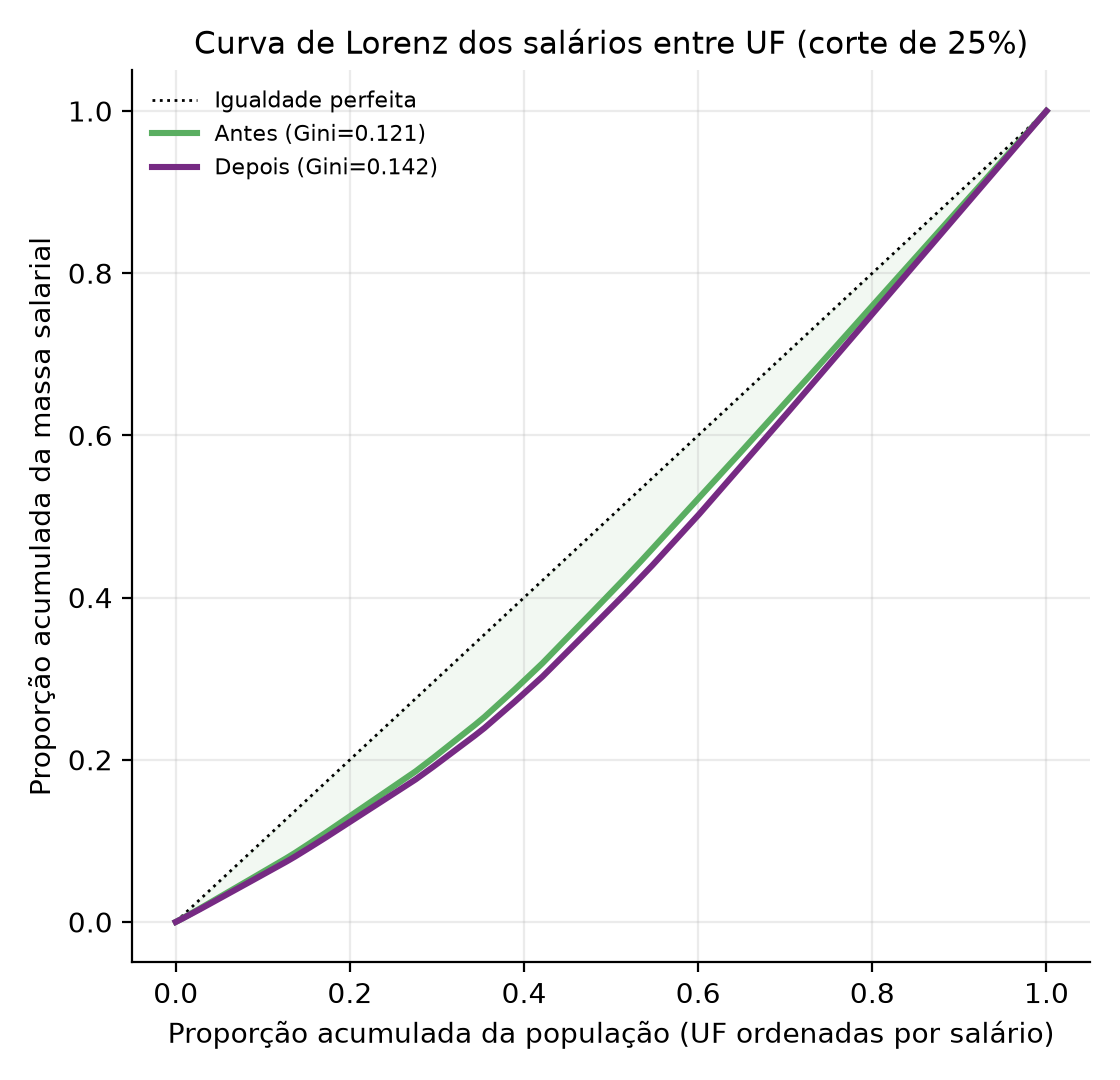
\includegraphics[width=\textwidth]{figures/lorenz.png}
\end{minipage}
\caption{Perda salarial por UF do corte de $1\%$ (esq.) e curva de Lorenz antes/depois do corte de $25\%$ (dir.)}
\label{fig:proj}
\fonte{Elabora\c{c}\~ao pr\'opria.}
\end{figure}

\begin{figure}[H]
\centering
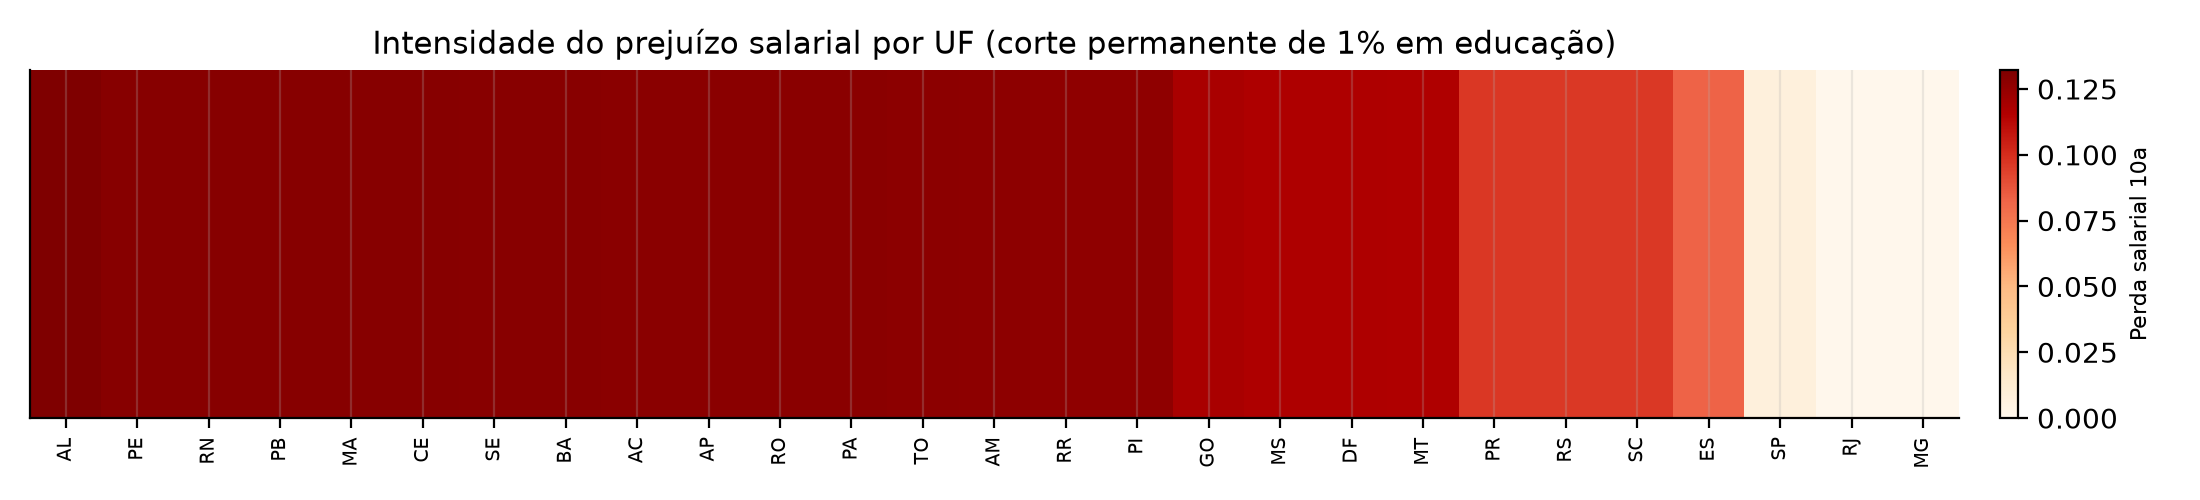
\includegraphics[width=\textwidth]{figures/mapa_calor_uf.png}
\caption{Intensidade do preju\'izo salarial por UF}
\label{fig:mapa}
\fonte{Elabora\c{c}\~ao pr\'opria.}
\end{figure}

\begin{table}[H]
\centering
\caption{Estados com maior perda salarial projetada (12 maiores)}
\label{tab:proj}
\small
\begin{tabular}{llrrr}
\toprule
UF & Região & Elast.\ EB & Perda sal.\ 10a & Perda sal.\ 20a \\
\midrule
AL & NE & 0,212 & 0,132 & 0,765 \\
PE & NE & 0,208 & 0,129 & 0,749 \\
RN & NE & 0,208 & 0,129 & 0,748 \\
PB & NE & 0,208 & 0,129 & 0,748 \\
MA & NE & 0,208 & 0,129 & 0,748 \\
CE & NE & 0,207 & 0,129 & 0,748 \\
SE & NE & 0,207 & 0,129 & 0,746 \\
BA & NE & 0,207 & 0,129 & 0,745 \\
AC & N & 0,206 & 0,128 & 0,744 \\
AP & N & 0,206 & 0,128 & 0,742 \\
RO & N & 0,206 & 0,128 & 0,742 \\
PA & N & 0,206 & 0,128 & 0,742 \\
\bottomrule
\end{tabular}

\fonte{Elabora\c{c}\~ao pr\'opria.}
\end{table}

% =============================================================================
\section{Resultados III: o corte aprofunda a desigualdade regional}\label{sec:res3}
% AUTHOR WRITES
% =============================================================================

\begin{figure}[H]
\centering
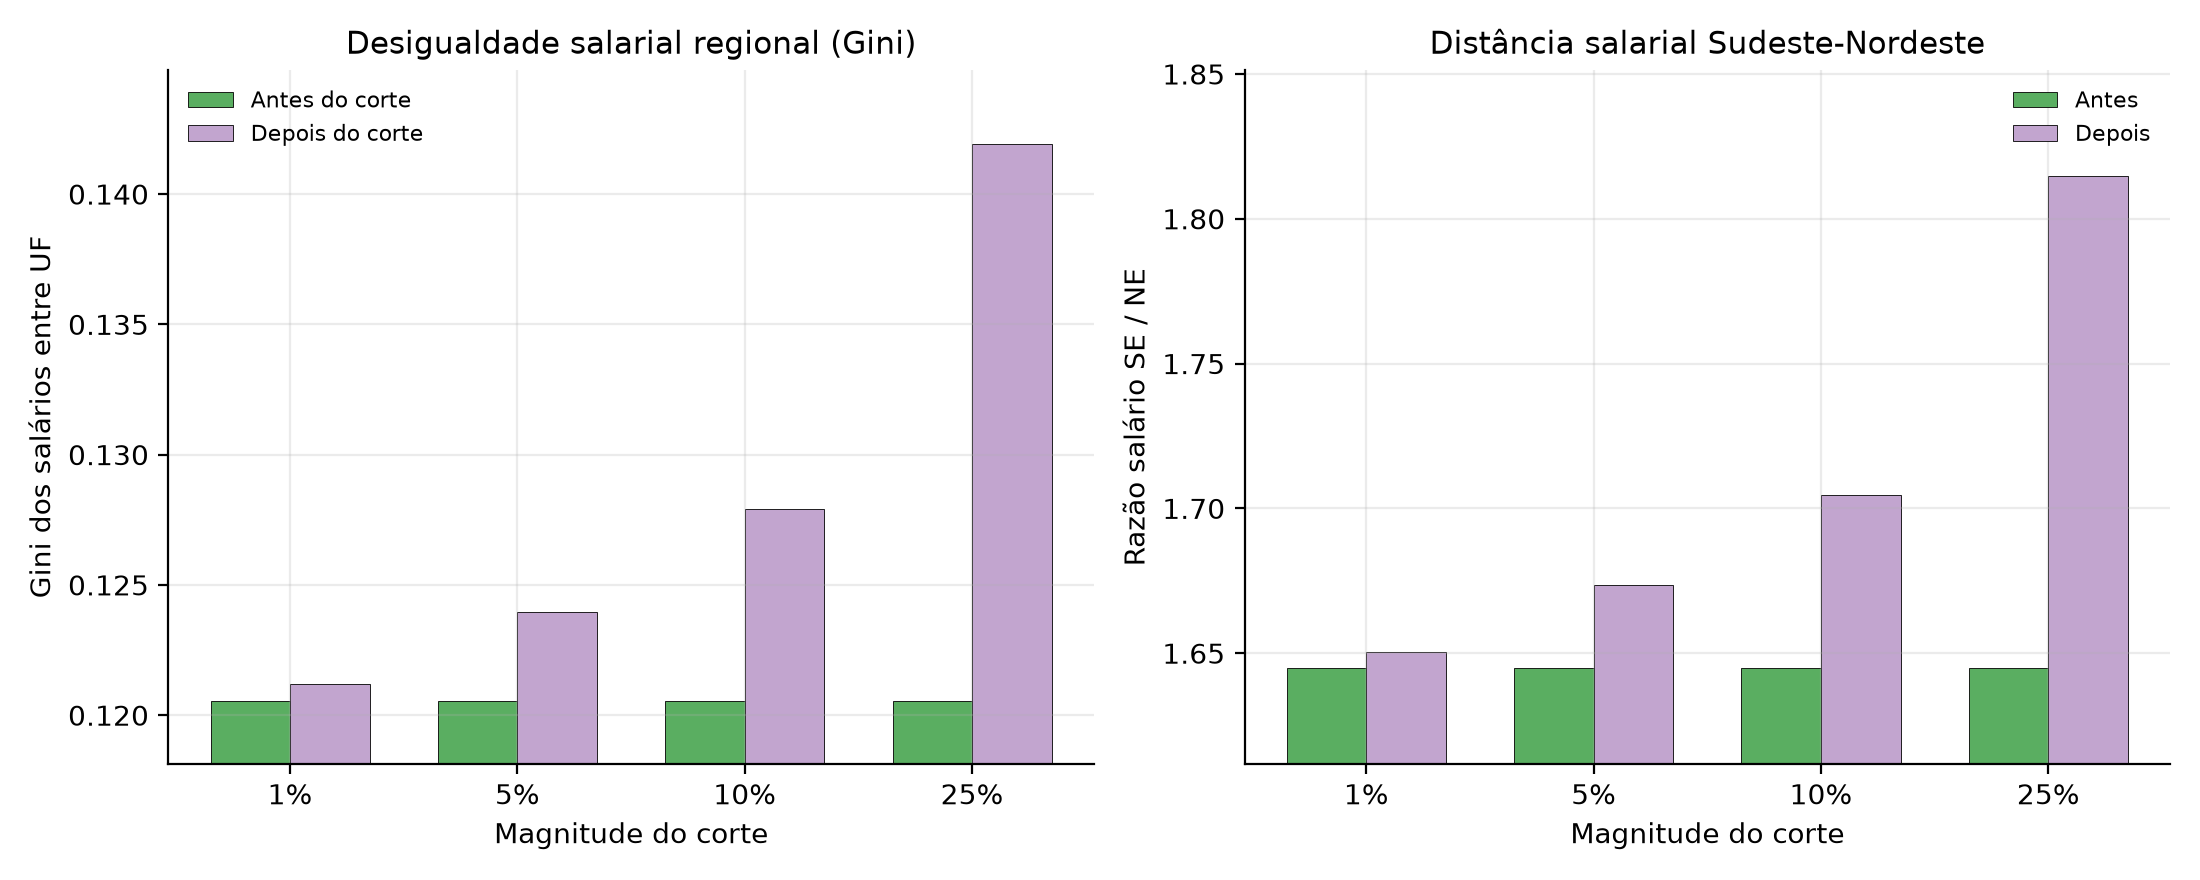
\includegraphics[width=\textwidth]{figures/desigualdade_gini.png}
\caption{Desigualdade regional antes/depois do corte: Gini entre UF (esq.) e raz\~ao SE/NE (dir.)}
\label{fig:gini}
\fonte{Elabora\c{c}\~ao pr\'opria.}
\end{figure}

\begin{table}[H]
\centering
\caption{Desigualdade regional por magnitude do corte}
\label{tab:desig}
\small
\begin{tabular}{lrrrrr}
\toprule
Corte & Gini antes & Gini depois & $\Delta$ Gini (\%) & SE/NE antes & SE/NE depois \\
\midrule
1\% & 0,1205 & 0,1212 & 0,53 & 1,645 & 1,650 \\
5\% & 0,1205 & 0,1240 & 2,83 & 1,645 & 1,674 \\
10\% & 0,1205 & 0,1279 & 6,10 & 1,645 & 1,705 \\
25\% & 0,1205 & 0,1419 & 17,72 & 1,645 & 1,815 \\
\bottomrule
\end{tabular}

\fonte{Elabora\c{c}\~ao pr\'opria. Gini e raz\~ao ponderados pela popula\c{c}\~ao (Censo 2022).}
\end{table}

\begin{table}[H]
\centering
\caption{Decomposi\c{c}\~ao de Theil da desigualdade salarial entre UF}
\label{tab:theil}
\small
\begin{tabular}{lrrr}
\toprule
Cenário & Theil total & Entre regiões & Dentro das regiões \\
\midrule
Antes do corte & 0,0270 & 0,0248 & 0,0022 \\
Após corte de 25\% & 0,0356 & 0,0334 & 0,0021 \\
Variação (\%) & 32,0 & 34,9 & -0,6 \\
\bottomrule
\end{tabular}

\fonte{Elabora\c{c}\~ao pr\'opria. Decomposi\c{c}\~ao entre e dentro de macrorregi\~oes.}
\end{table}

\begin{figure}[H]
\centering
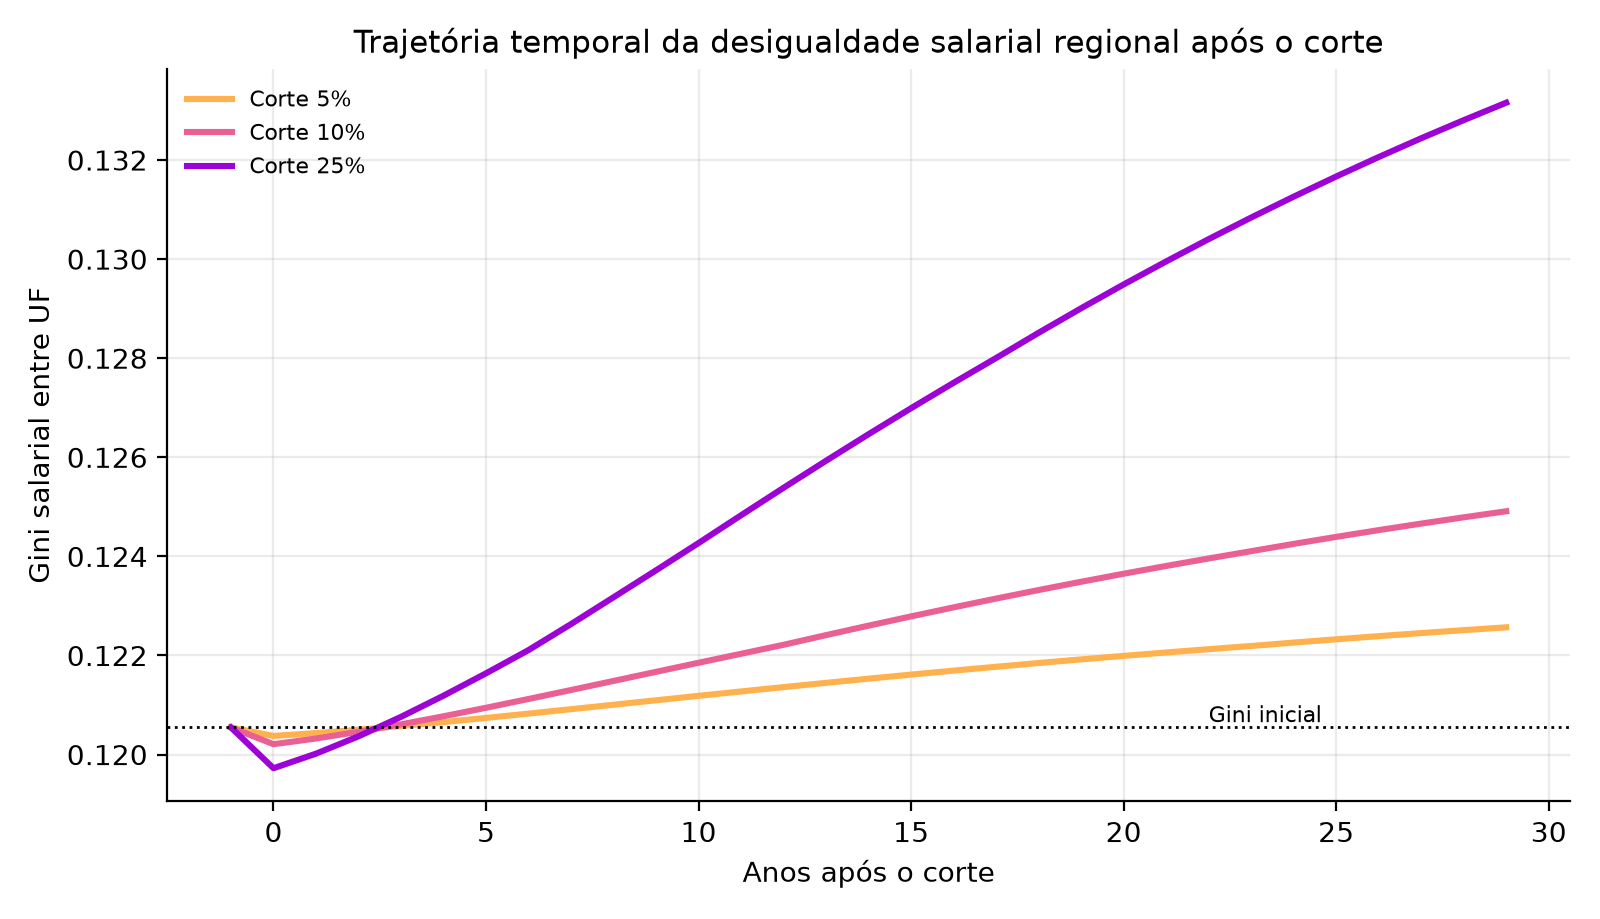
\includegraphics[width=0.82\textwidth]{figures/gini_trajetoria.png}
\caption{Trajet\'oria temporal do Gini salarial entre UF ap\'os o corte}
\label{fig:ginitraj}
\fonte{Elabora\c{c}\~ao pr\'opria.}
\end{figure}

% =============================================================================
\section{Discuss\~ao e conclus\~ao}
% AUTHOR WRITES
% =============================================================================

\section*{Disponibilidade de dados e c\'odigo}
% AUTHOR WRITES

\bibliography{referencias}
\end{document}
